\subsubsection{Gerando e Medindo NBTI}
\label{sec:GerandoNbti}

Muitos estudos já foram realizados para determinar em que condições o NBTI ocorre com mais facilidade em circuitos CMOS.

O fenômeno NBTI normalmente ocorre em transistores do tipo p operando com tensão de gate negativa em temperaturas variando de 100ºC a 250ºC \cite{Davidovic}. Os campos elétricos devem ser na faixa dos 6MV/cm, valores encontrados durante o \textit{burn-in} do componente, porém com transistores cada vez menores, esses campos podem ocorrer durante a operação normal de dispositivos de alta performance \cite{Schroder}. A Figura \ref{fig:CampoEletricoAno} mostra o aumento do campo elétrico que atravessa o óxido em transistores CMOS ao longo dos anos.

\begin{figure}[H]
    \centering
    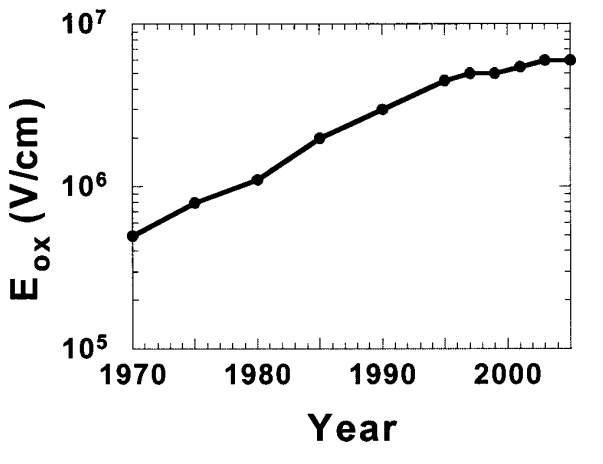
\includegraphics[scale=0.5]{figures/ReferencialTeorico/CampoEletricoAno.png}
    \caption{Campo elétrico no óxido em dispositivos CMOS ao longo dos anos. Fonte: \cite{Schroder}}
    \label{fig:CampoEletricoAno}
\end{figure}

% Typical stress temperatures lie in the 100– 250 °C range with oxide electric fields typically below 6 MV/cm, i.e., fields below those that lead to hot carrier degradation. Such fields and temperatures are typically encountered during burn in, but are also approached in highperformance ICs during routine operation.

Para aplicar o efeito de NBTI no dispositivo ensaiado no trabalho \cite{Davidovic}, os pesquisadores o estressaram por 2000 horas, aplicando tensões negativas de 30 a 45V no gate (com fonte e dreno aterrados) em uma temperatura de variando de 125 a 175ºC.

O trabalho de \cite{Bhardwaj} desenvolveu um modelo preditivo para NBTI em dispositivos CMOS de nó tecnológico de 45nm, que alcançou estimativas precisas da degradação em longo prazo da tensão de \textit{threshold} de transistores PMOS devido ao fenômeno.

Um outro trabalho \cite{Grossi}, realizou simulações para analisar os efeitos do BTI em amplificadores operacionais, e viu que o ganho DC, a frequência de corte e o \textit{slew rate} são significativamente degradados em AMPOPs operando em malha aberta. Já para Ampops operando com realimentação negativa apenas a frequência de corte mostrou uma degradação significativa.

Alguns trabalhos, inclusive, realizaram estudos dos efeitos de NBTI em osciladores em anel. Um deles \cite{Lorenz} mostra uma degradação de 5\% com 144 horas de exposição à 125°C. Já outro \cite{Sato}, que estudou métodos para diminuir o efeito de NBTI em osciladores em anel, resultou uma degradação de 0,25\%, com 42 horas de exposição, porém à apenas 85°C. Um terceiro trabalho \cite{Linder} propõe topologias de osciladores em anel que permitem estudar em separado os efeitos do PBTI, nele foi medida um degradação de 1,8\% considerando apenas o PBTI, 2,2\% considerando apenas o NBTI e 3,9\%  considerando apenas os dois efeitos combinados tendo sido realizado um estresse de 2 horas e 47 minutos (10000 segundos) segundos à 125°C.

Esses três trabalhos avaliaram a degradação causada pelo NBTI através da diminuição da frequência de osciladores em anel. Isso é viável, pois a variação da tensão de \textit{treshold} causada pelo NBTI aumentará o tempo de propagação dos transistores dos circuitos, aumentando o período de oscilação. 